\section{Perceptron}
\subsection{And gate}
\begin{tabular}{c | c | c | c}
	x1 & x2 & $w_{0}+ w_{1}x_{1}+ w_{2}x_{2}$ & y  \\
	\hline
	0  & 0  & -2 + 1 * 0 + 1 * 0 = -2 < 0     & -1 \\
	\hline
	0  & 1  & -2 + 1 * 0 + 1 * 1 = -1 < 0     & -1 \\
	\hline
	1  & 0  & -2 + 1 * 1 + 1 * 0 = -1 < 0     & -1 \\
	\hline
	1  & 1  & -2 + 1 * 1 + 1 * 1 = 0 = 0      & 1  \\
\end{tabular}

\subsection{Or gate}
\begin{tabular}{c | c | c | c}
	x1 & x2 & $w_{0}+ w_{1}x_{1}+ w_{2}x_{2}$ & y  \\
	\hline
	0  & 0  & -1 + 1 * 0 + 1 * 0 = -1 < 0     & -1 \\
	\hline
	0  & 1  & -1 + 1 * 0 + 1 * 1 = 0 $\geq$ 0 & 1  \\
	\hline
	1  & 0  & -1 + 1 * 1 + 1 * 0 = 0 $\geq$ 0 & 1  \\
	\hline
	1  & 1  & -1 + 1 * 1 + 1 * 1 = 1 $\geq$ 0 & 1  \\
\end{tabular}

\subsection{Not gate}
\begin{tabular}{c | c | c}
	x1 & $w_{0}+ w_{1}x_{1}+ w_{2}x_{2}$ & y  \\
	\hline
	0  & 0 - 1 * 0 = 0 $\geq$ 0          & 1  \\
	\hline
	1  & 0 - 1 * 1 = -1 < 0              & -1 \\
\end{tabular}

\subsection{Xor gate}
Is not linearly separable because the function is not convex.

\subsection{Same gate with multiple perceptron}
x1 SAME x2 = (NOT x1 AND not x2) OR (x1 AND x2) But now the intermediate perceptron
need to handle -1 and 1 inputs. New XOR:
\begin{tabular}{c | c | c | c}
	x1 & x2 & $w_{0}+ w_{1}x_{1}+ w_{2}x_{2}$ & y  \\
	\hline
	-1 & -1 & 1 + 1 * -1 + 1 * -1 = -1 < 0    & -1 \\
	\hline
	-1 & 1  & 1 + 1 * -1 + 1 * 1 = 1 $\geq$ 0 & 1  \\
	\hline
	1  & -1 & 1 + 1 * 1 + 1 * -1 = 1 $\geq$ 0 & 1  \\
	\hline
	1  & 1  & 1 + 1 * 1 + 1 * 1 = 3 $\geq$ 0  & 1  \\
\end{tabular}
\subsection{Perceptron with tanh}
\begin{tabular}{c | c | c| c}
	Operator & $w_{0}$ & $w_{1}$ & $w_{2}$ \\
	\hline
	AND      & -300    & 200     & 200     \\
	\hline
	OR       & -100    & 200     & 200     \\
	\hline
	NOT      & 100     & -200     \\
\end{tabular}

\section{Centering and Ridge regression}
$\mathcal{L}(w,b)=(Xw +b1-y)^{T}(Xw +b1-y)+\lambda w^{T}w$\\
$=w^{T}X^{T}Xw+w^{T}X^{T}b1-w^{T}X^{T}y +[(b1)^{T}Xw]+[(b1)^{T}(b1)]-[(b1)^{T}y]-
y^{T}Xw-y^{T}b1+y^{T}y+\lambda w^{T}w$\\ Because $X^{T}c1=(d1)^{T}X=0$ when $\frac{1}{N}
\sum_{i=1}^{N}x_{i}= 0$ then $w^{T}X^{T}b1=w^{T}*0=0$\\ Also: $(b1)^{T}(b1) = Nb^{2}$,
so after resolving terms:\\
$=w^{T}X^{T}Xw-y^{T}Xw +Nb^{2}-y^{T}b1-y^{T}Xw-y^{T}b1 +y^{T}y +\lambda w^{T}w$\\
$=w^{T}X^{T}Xw-2y^{T}Xw +Nb^{2}-2y^{T}b1+y^{T}y +\lambda w^{T}w$\\
$\nabla{w}\mathcal{L}_{ridge}=2X^{T}Xw-2X^{T}y+2\lambda w$\\ Because $\nabla_{b}(
2y^{T}(b1))=2\sum_{i=1}^{N}y_{i}$\\
$\nabla{b}\mathcal{L}_{ridge}=2N b-2\sum_{i=1}^{N}y_{i}$\\ Set $\nabla{w}\mathcal{L}
_{ridge}$ to 0:\\ Take $X^{T}y$ to the other side and extract w:\\ $w=(X^{T}X+\lambda
I_{D})^{-1}X^{T}y$\\
\section{Newtons method for ridge regression}
$\nabla{w}\mathcal{L}_{ridge}=2X^{T}Xw-2X^{T}y+2\lambda w$\\ $H_{ridge}=\nabla_{w}
(\nabla{w}\mathcal{L}_{ridge})=2(X^{T}X+\lambda I_{D})$\\ Newtons method:\\
$w_{t+1}=w_{t}-\eta H^{-1}\nabla f(w_{t})$\\ $=w_{t}-2^{-1}(X^{T}X+\lambda I_{D})
^{-1}2((X^{T}X+\lambda I_{D})w_{t}-X^{T}y)$\\
$=w_{t}-(X^{T}X+\lambda I_{D})^{-1}((X^{T}X+\lambda I_{D})w_{t}-X^{T}y)$\\ Because
$(X^{T}X+\lambda I_{D})^{-1}*(X^{T}X+\lambda I_{D})=1$\\
$=w_{t}-(w_{t}-( X^{T}X+\lambda I_{D})^{-1}X^{T}y)$
\section{Neuronal nets}
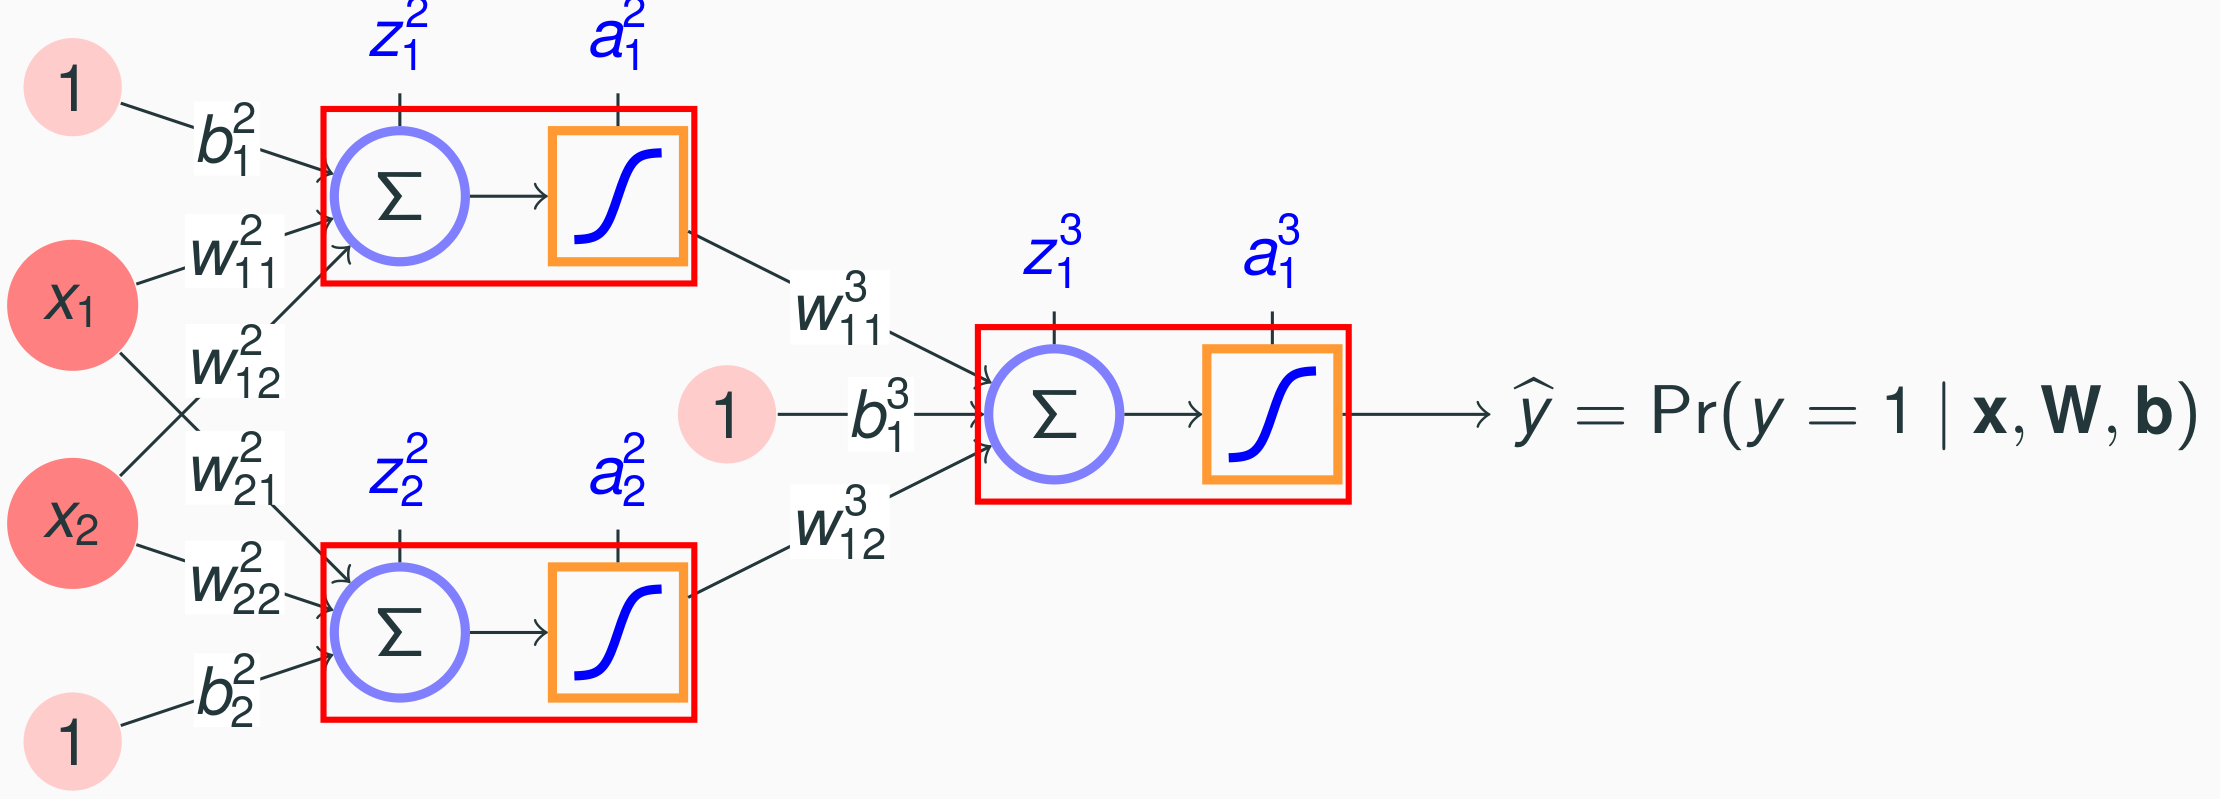
\includegraphics[width=65mm]{sections/assets/perceptron}
Pre-activation 1:
\[
	z^{2}=\left[
	\begin{matrix}
		w_{11}^{2}x_{1}+ w_{12}^{2}x_{2}+ b_{1}^{2} \\
		w_{21}^{2}x_{1}+ w_{22}^{2}x_{2}+ b_{2}^{2} \\
	\end{matrix}\right]
\]
Activation 1 (here with tanh):
\[
	a^{2}= \tanh(z^{2})=\left[
	\begin{matrix}
		\tanh(w_{11}^{2}x_{1}+ w_{12}^{2}x_{2}+ b_{1}^{2}) \\
		\tanh(w_{21}^{2}x_{1}+ w_{22}^{2}x_{2}+ b_{2}^{2}) \\
	\end{matrix}\right]
\]
Pre-activation 2:\\
$z^{3}=[w_{11}^{3}a_{1}^{2}+ w_{12}^{3}a_{2}^{2}+ b_{1}^{3}]$\\ Activation 2:\\ $a
^{3}=\sigma(z^{3})=[\sigma(w_{11}^{3}a_{1}^{2}+ w_{12}^{3}a_{2}^{2}+ b_{1}^{3})]$\\
Define a loss function, e.g. cross entropy loss: $l(a^{3}, y) = -(y \log(a_{1}^{3}
) + (1-y)\log(1-a_{1}^{3}))$\\
$\frac{dl}{da_{1}^{3}}=-\left[\frac{y}{a_{1}^{3}}+\frac{1-y}{1-a_{1}^{3}}*(-1)\right
]=-\frac{y(1-a_{1}^{3})-(1-y)a_{1}^{3}}{a_{1}^{3}(1-a_{1}^{3})}=\frac{a_{1}^{3}-
y}{a_{1}^{3}(1-a_{1}^{3})}$\\ $\frac{da^{3}}{dz^{3}}=\sigma'(z_{1}^{3})=a_{1}^{3}
(1 - a_{1}^{3})$\\
$\frac{dl}{dz^{3}}=\frac{dl}{da_{1}^{3}}\frac{da_{1}^{3}}{dz^{3}}=\left[ \frac{a_{1}^{3}-
y}{a_{1}^{3}(1-a_{1}^{3})}\right] \left[ a_{1}^{3}(1 - a_{1}^{3}) \right] = a_{1}
^{3}- y$\\ $z^{3}=W^{3}a^{2}+b^{3}$, so $\frac{dz^{3}}{da^{2}}=W^{3}$\\ $\tanh(t
)=\frac{e^{t}-e^{-t}}{e^{t}+e^{-t}}$ and $\tanh'(t)=1-\tanh(t)^{2}$\\
$\frac{dl}{dz^{2}}=\frac{dl}{dz^{3}}\frac{dz^{3}}{da^{2}}\frac{da^{2}}{dz^{2}}=[a
_{1}^{3}-y]W^{3}\left[
\begin{matrix}
	1-(a_{1}^{2})^{2} & 0                 \\
	0                 & 1-(a_{2}^{2})^{2}
\end{matrix}
\right]$
\section{Requirements on N for linear regression}
The rank of X is D\\ The rank of $X^{T}$ is D\\ $D \leq N$\\